\documentclass{article}
\usepackage{amsmath}
\usepackage{amsfonts}
\usepackage{tikz}
\usetikzlibrary{calc}

\begin{document}

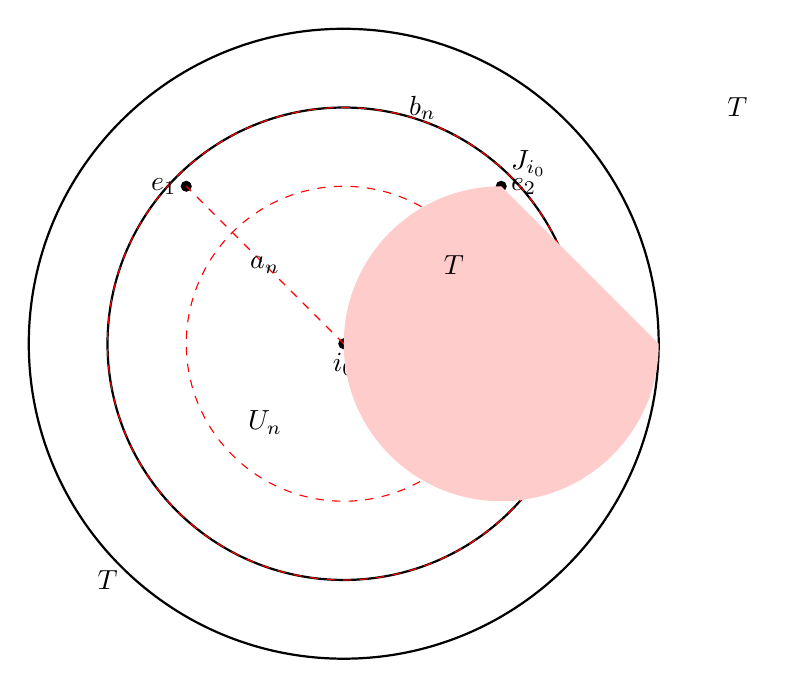
\begin{tikzpicture}[scale=2]
    % Define coordinates
    \coordinate (e1) at (-1, 1);
    \coordinate (e2) at (1, 1);
    \coordinate (i0) at (0, 0);
    
    % Draw circles
    \draw[thick] (0,0) circle (1.5);
    \draw[thick] (0,0) circle (2);
    \draw[dashed, red] (0,0) circle (1);
    \draw[dashed, red] (0,0) circle (1.5);
    
    % Draw points
    \fill (e1) circle (1pt) node[left] {$e_1$};
    \fill (e2) circle (1pt) node[right] {$e_2$};
    \fill (i0) circle (1pt) node[below] {$i_0$};
    
    % Draw lines
    \draw[dashed, red] (i0) -- (e2);
    \draw[dashed, red] (i0) -- (e1);
    
    % Fill region J_{i_0}
    \fill[red!20] ($(i0)!1!(e2)$) arc (90:360:1) -- cycle;
    \node at ($(i0)!1!(e2)$) [above right] {$J_{i_0}$};
    
    % Labels
    \node at (-1.5, -1.5) {$T$};
    \node at (2.5, 1.5) {$T$};
    \node at (0.7, 0.5) {$T$};
    \node at (0.5, 1.5) {$b_n$};
    \node at (-0.5, 0.5) {$a_n$};
    \node at (-0.5, -0.5) {$U_n$};
\end{tikzpicture}

\end{document}